\documentclass[useAMS, usenatbib]{aastex}
\usepackage{cite,natbib}
\usepackage{epsfig}
\usepackage{cases}
\usepackage[section]{placeins}
\usepackage{graphicx, subfigure}
\usepackage{color}

\title{Detecting periodic signals in K2 data}

\begin{document}

\date{Draft version 2015 24th of February}
\maketitle

% Aims
From pulsating stars to transiting exoplanets, the search for periodic signals
in {\it K2} data is relevent to a long list of scientific goals.
Systematics affecting {\it K2} light curves due to the decreased pointing
precision of the space craft inhibit the easy extraction of periodic signals
from the data.
We here develop a method for producing periodograms of K2 light curves that
are insensitive to pointing-induced systematics.
% Methods
Sine-fitting periodogram methods use a generative model to find the frequency
of the sine wave that best describes the data.
We extend this principle by including systematic trends in our generative
model as well as a sum of sines and cosine functions over a grid of
frequencies.
% Results
Our method is able to produce periodograms with significantly reduced
systematic features, such that we can recover acoustic oscillations in giants
without the need for any detrending.
Whilst this method performs extremely well in the high part of frequency space,
relevent for giant asteroseismology, it is not optimised for measuring stellar
rotation periods.
This is due to the fact that some common trends between stars vary on
timescales similar to rotation periods.

\section{Introduction}
\label{Introduction}

With the failure of {\it Kepler}'s third reaction in 2012, the space craft was
repurposed, and in 2014 the {\it K2} mission began.
The excellent precision achieved by the original {\it Kepler} mission relied on extremely precise pointing, for which three reaction wheels were crucial.
Now, with just two reaction wheels, it is only possible to point the telescope
at fields lying in the ecliptic plane, using the Solar wind to stabilise
the space craft, with reduced precision.
The telescope is scheduled to observe n ecliptic fields for $\sim$3 months at a
time over the next n years.
Within these fields there are thousands of variable stars, rotating stars,
pulsating stars and exoplanet hosts.
Developing methods for the extraction of periodic information from K2 light
curves, despite the reduced pointing precision is therefore extremely
important.

The original {\it Kepler} mission provided a huge set of  light curves with
periodic behaviour on timescales ranging from a few minutes to a few months.
The field of asteroseismology was enormously advanced by the excellent
precision of {\it Kepler} data and the short integration times acheivable for
a few hundred targets.
Around 600 Solar-like oscillators, which pulsate on $\sim$5 minute timescales,
were observed in short cadence mode.
The asteroseismic pulsations of giant stars lie below the Nyquist frequency set
by the sampling rate of long cadence {\it Kepler} data
These stars oscillate on, of order, hour-long timescales, below the Nyquist
frequency of 283 $\mu$Hz set by the 28.5 minute cadence.
Fundamental stellar parameters---in some cases, extremely precise ones---can
be calculated for {\it Kepler} asteroseismic stars from the power spectra of
their light curves.
The Fast Fourier Transform (FFT) and sine-fitting periodogram are fundamental
tools in the asteroseismic toolbox.
Asteroseismic analysis of {\it Kepler} data is traditionally conducted using
detrended light curves.
For short cadence data, this detrending method is described in
\citet{Garcia2011}.

Stellar rotation periods can be extracted from the high precision photometry
of {\it Kepler}; active regions on the surface of a rotating star produce
periodic variations in flux.
Stellar rotation is a field of active interest as the rotation period of
a star can be used to infer its age (CITATIONS), and could reveal dynamical
interations with companion stars or planets (CITATIONS).
Rotation periods are also useful for {\it Kepler} exoplanet characterization.
Active regions can produce variability in radial velocity as well as
photometry and can masquerade as planetary signals.
It is therefore extremely useful to be able measure the rotation period of the
star directly from the light curve.
Current methods for measuring rotation periods from {\it Kepler} light curves
include periodogram \citep[e.g.][]{Reinhold2013}, AutoCorrelation Function
(ACF) \citep{McQuillan2013} and wavelet \citep[e.g.][]{Garcia2014} analysis,
or some combination thereof.
Stellar variability is not typically sinusoidal, therefore sine-fitting
periodograms are not perfectly suited for measuring rotation periods.
For this reason, the ACF method is often favoured over the periodogram method.
However, because autocorrelation is performed on the data, not a generative
model, we cannot use autocorrelation techniques on non-detrended {\it K2} data.
A quasi-periodic Gaussian process is a much better effective model for stellar
variability, however we are not only concerned with stellar rotation and choose
to focus on the more generally applicable sine-wave periodogram, leaving the
Gaussian process for future work.

Aside from asteroseismology and stellar rotation there are many other fields
of research that use light curve periodicity studies.
These include searching for eclipsing binaries, variable stars and exoplanets,
even studying white dwarfs and AGN.
The development of tools for extracting periodic information from {\it K2}
data is essential if it is to be as revolutionary in time-domain
astronomy as its ancestor was.

\section{Method}
\label{Method}

The method implemented in this paper is an extention of the planet-search
algorithm developed by \citet{Foreman-Mackey2015} (hereafter FM15).
All the stars observed by {\it Kepler} move on the CCD in the same way and
therefore the systematics affecting each individual star's light curve have
shared properties.
The FM12 method utilizes the fact that pointing-induced systematics are shared
across stars and decomposes the trends into a set of `eigen light curves'
using Principle Component Analysis (PCA).
This method is similar to that used to produce PDC-MAP data for the original
{\it Kepler} mission \citep[][]{Stumpe2012, Smith2012}.
Those eigen light curves can then be used to model any campaign 1 {\it }light
curve with an arbitrary physical model.
FM15 downloaded the target pixel files for all stars observed in campaign 1;
21,703 in total.
The position of each star was predicted using the world coordinate system and
10 circular apertures placed around the star with radii varying from 1 to
5 pixels in steps of 0.5 pixels.
Following the procedure of \citet{Vanderburg2014}, the aperture producing the
light curve with the lowest CDPP with a 6 hour window \citet{Christiansen2012}
was selected.
PCA was then performed on the full set of targets in order to produce `eigen
light curves.
FM15 used 150 of these eigen light curves with a transit model in order to
search for exoplanet candidates without the need for a `detrending' step.
The likelihood of the data, conditioned on their eigen-light-curve-plus-transit
model was calculated over a fine grid of periods and transit depths, resulting
in the detection of 36 new exoplanet candidates.
We use exactly the same technique to find periodic signals in {\it K2} data,
where, instead of a transit model, we use a sum of sine and cosine functions.

\section{Application to asteroseismology}

An example Lomb-Scargle periodogram\footnote{All Lomb-Scargle periodograms
produced in this project were calculated using the gatspy Python module:
https://github.com/astroML/gatspy/tree/master/gatspy/periodic}
of the raw {\it K2 photometry} for EPIC 201211472 is shown in figure
\ref{fig:raw}.
The peaks at 47 $\mu$Hz and its harmonics are produced by the regular $\sim$
6 hour thruster fires that repoint the spacecraft.
These peaks are also present in periodograms of the \citet{Vanderburg2014}
light curves.
The presence of systematic signals at these timescales are problematic for
asteroseismic analysis.
It is possible to remove these signals by `prewhitening' the data, i.e.
removing a sine wave at that frequency from the data, however no such
procedure is necessary for our method.

\begin{figure*}
\begin{center}
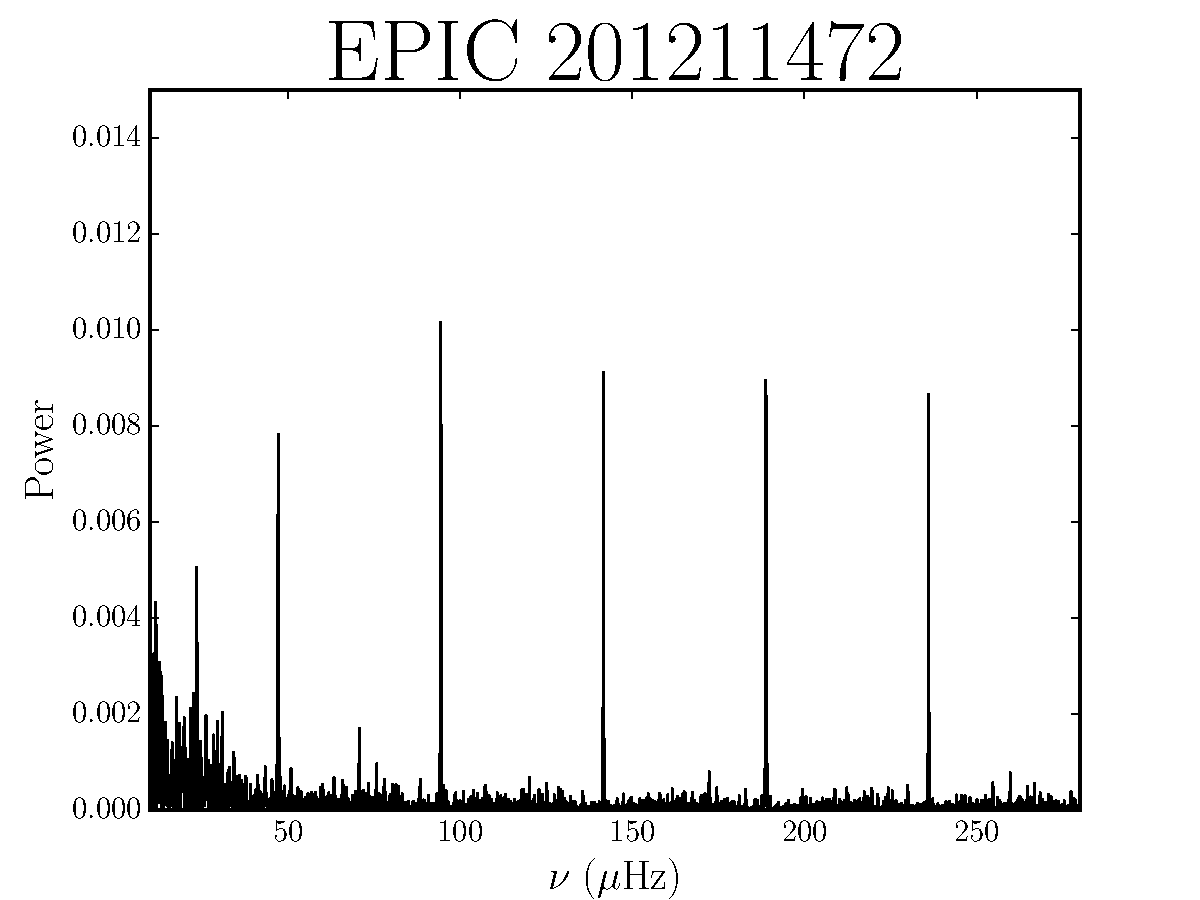
\includegraphics[width=6in, clip=true]{raw_201211472.pdf}
\caption{Lomb-scargle periodogram of the raw {\it K2 photometry for
	EPIC 201211472.}
\label{fig:raw}
\end{center}
\end{figure*}

We selected long cadence targets from the GO1059 proposal: "Galactic
Archaeology on a grand scale" (PI: Stello, D.) in order to test our method.
Figures \ref{fig:1} to \ref{fig6} show example power spectra of 6 targets for
which we detect pulsations.

\begin{figure}
\begin{center}
	\subfigure[]{
            \label{fig:1}
	    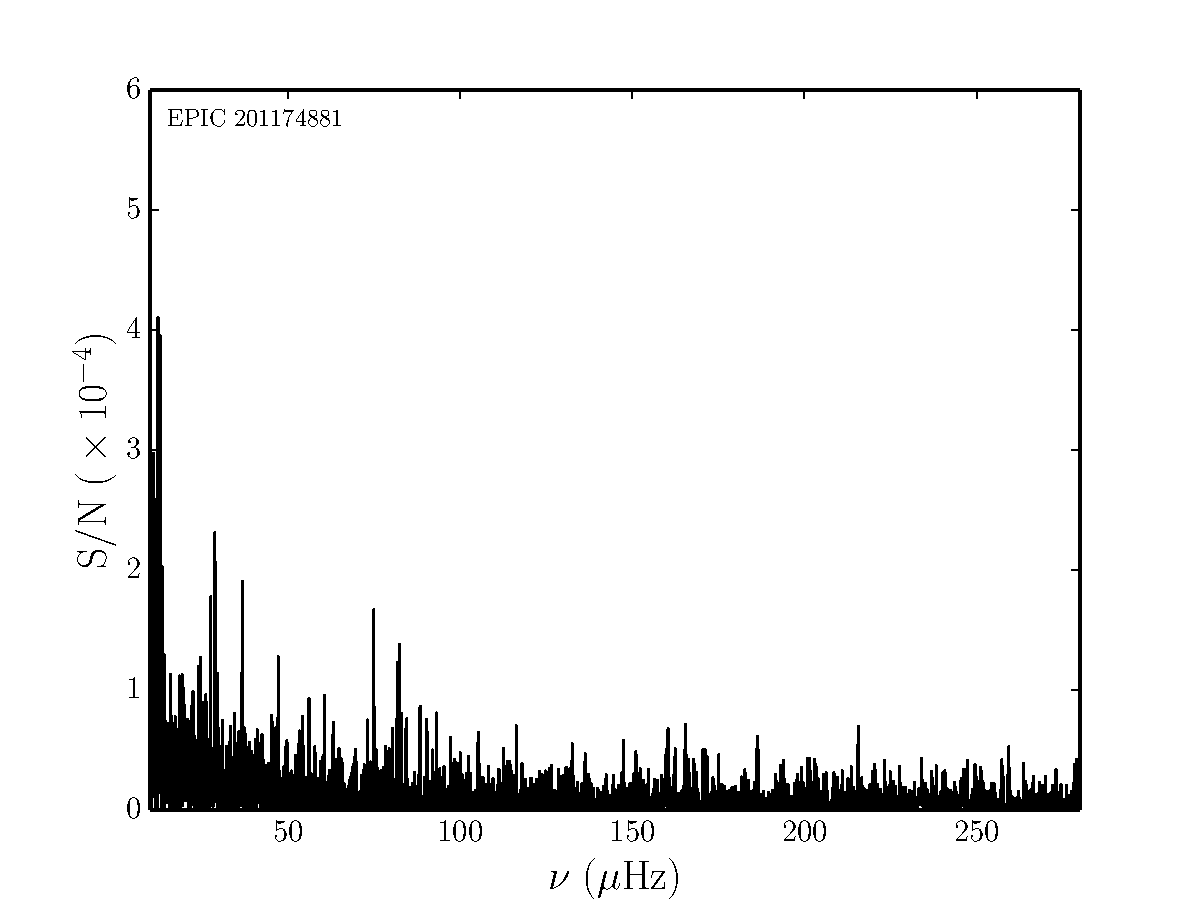
\includegraphics[width=3in]{201174881.pdf}
        }
	\subfigure[]{
            \label{fig:2}
	    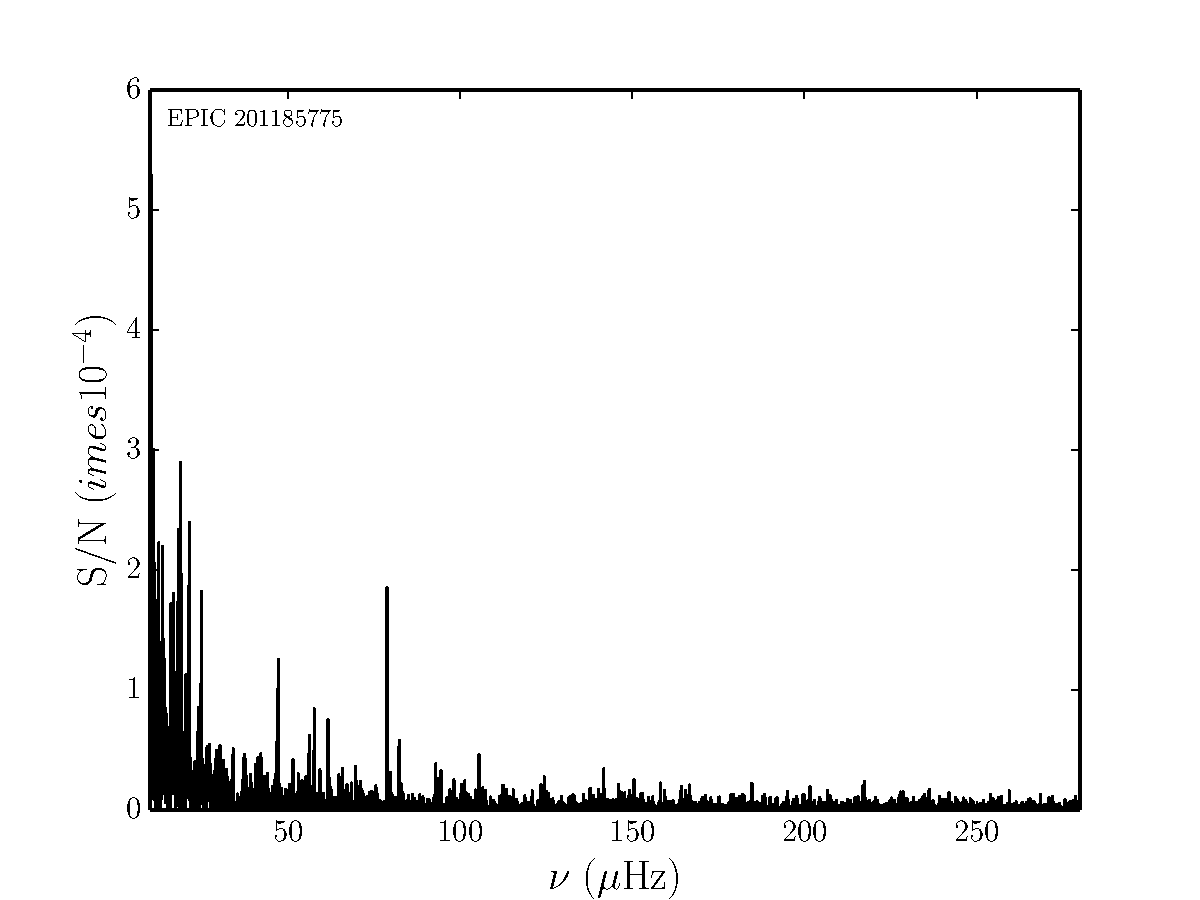
\includegraphics[width=3in]{201185775.pdf}
        }
	\subfigure[]{
            \label{fig:3}
	    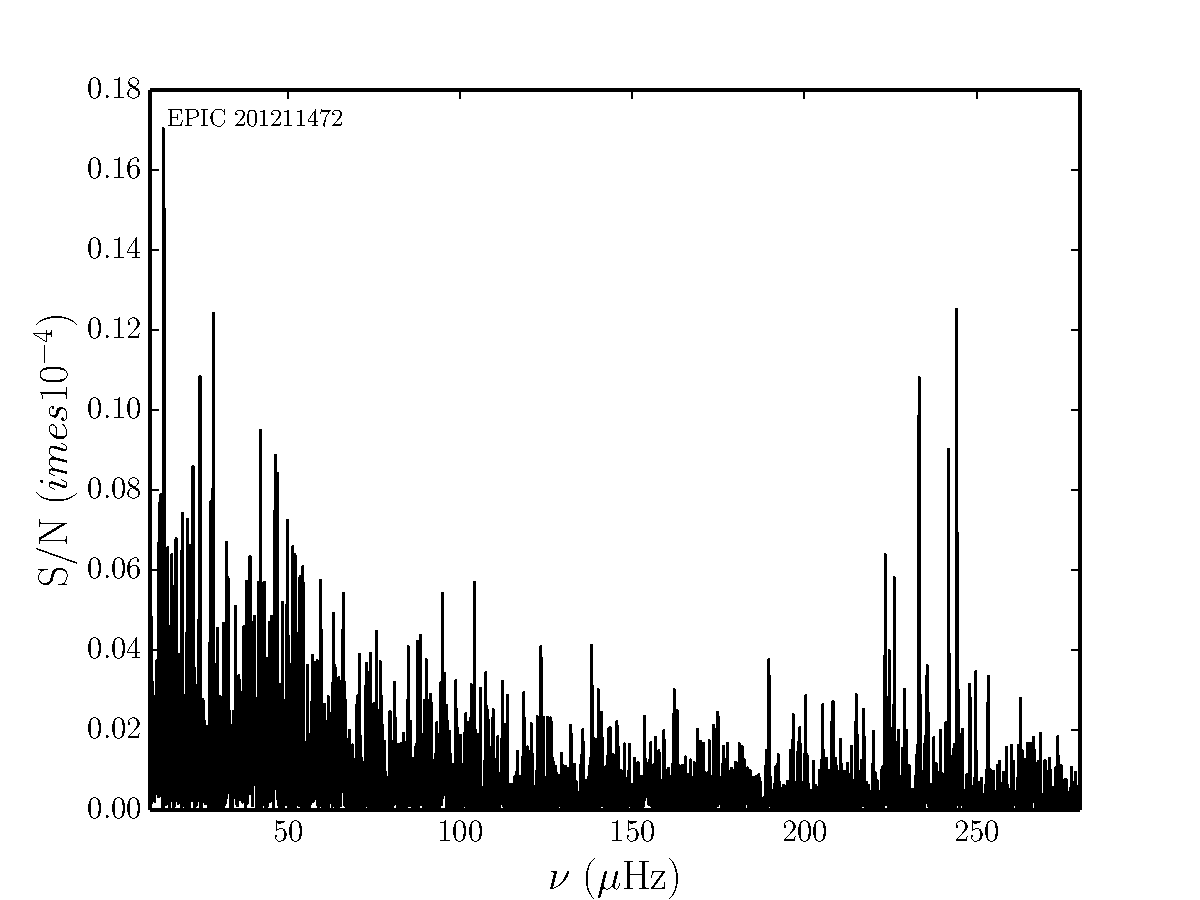
\includegraphics[width=3in]{201211472.pdf}
        }
	\subfigure[]{
            \label{fig:4}
	    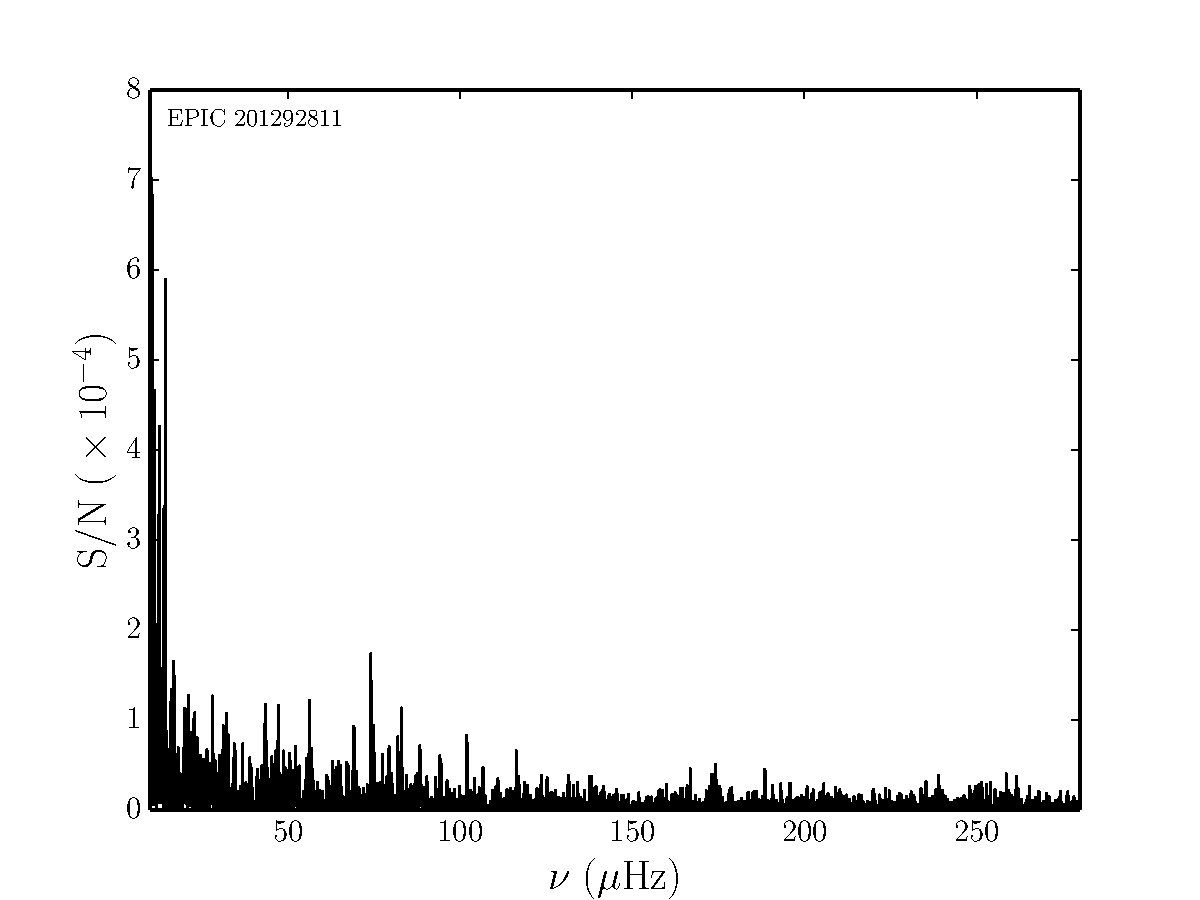
\includegraphics[width=3in]{201292811.pdf}
        }
	\subfigure[]{
            \label{fig:5}
	    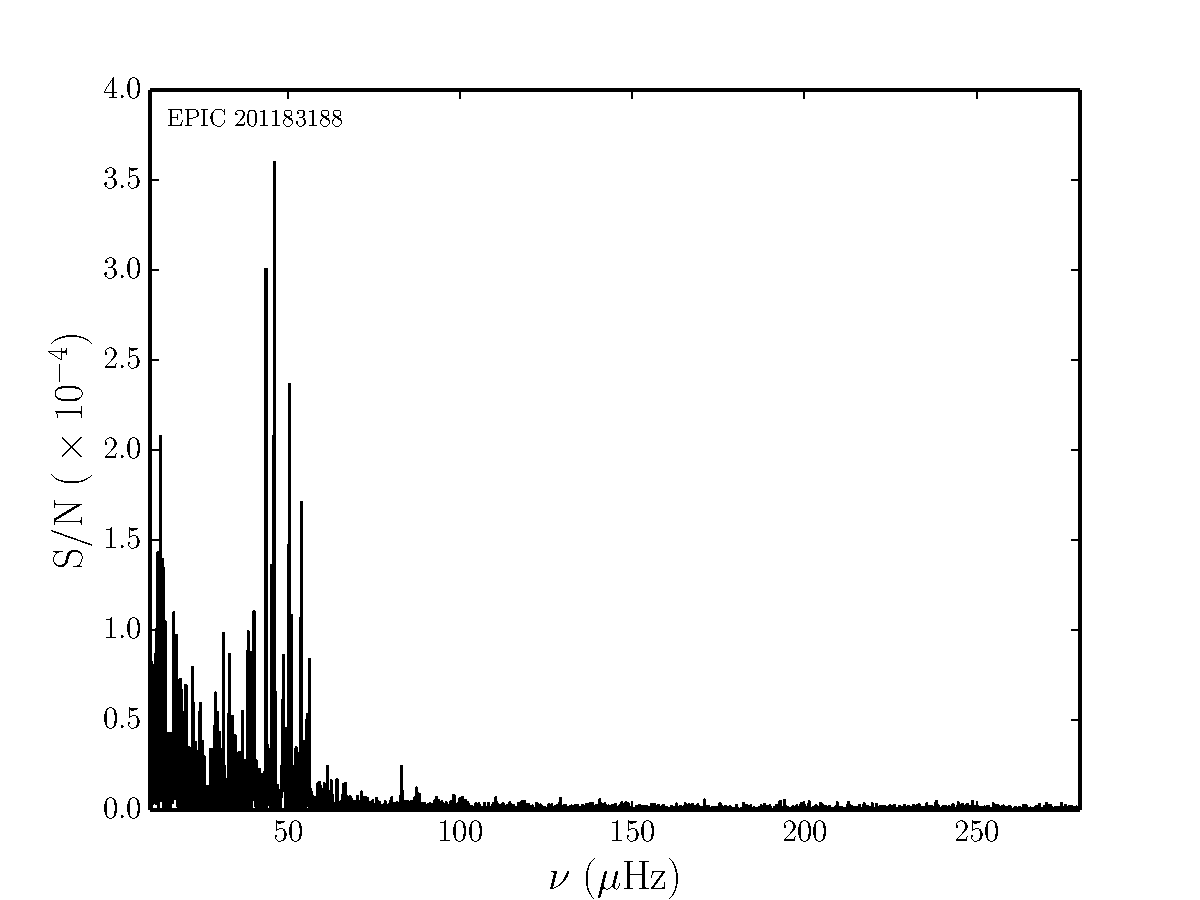
\includegraphics[width=3in]{201183188.pdf}
        }
	\subfigure[]{
            \label{fig:6}
	    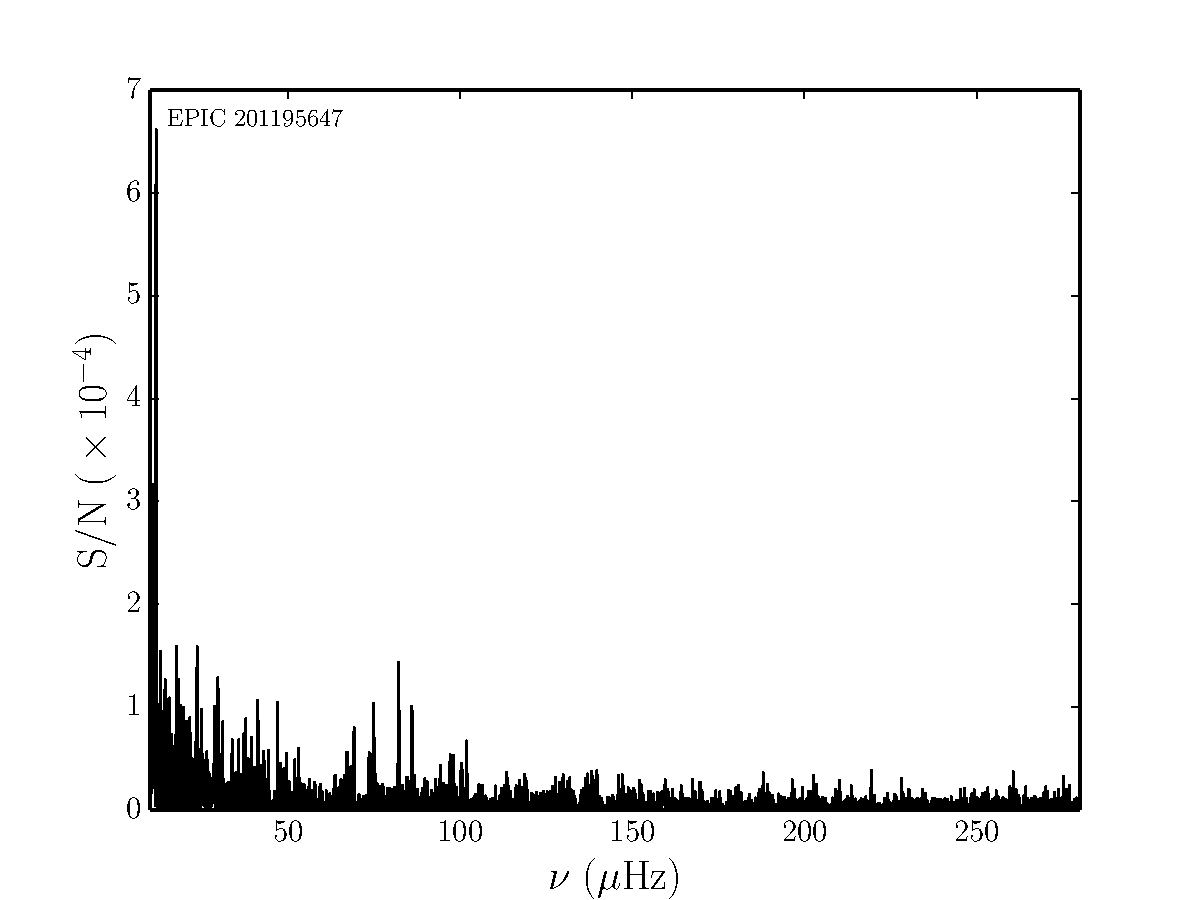
\includegraphics[width=3in]{201195647.pdf}
        }
% 	\subfigure[]{
%             \label{fig:7}
% 	    \includegraphics[width=3in]{201272670.pdf}
%         }
    \end{center}
    \caption{Power spectra of 6 long cadence {\it K2} giants with pulsations.
\label{fig:astero_examples}}
\end{figure}

These periodograms do not show the

\subsection{Flicker}

\section{Application to stellar rotation}
The top panel of figure \ref{fig:rotation_poster_child} shows the light curve
of an active, rotating star, EP201317002.
This light curve has been detrended using the method of
\citet{Vanderburg2014}.

\begin{figure*}
\begin{center}
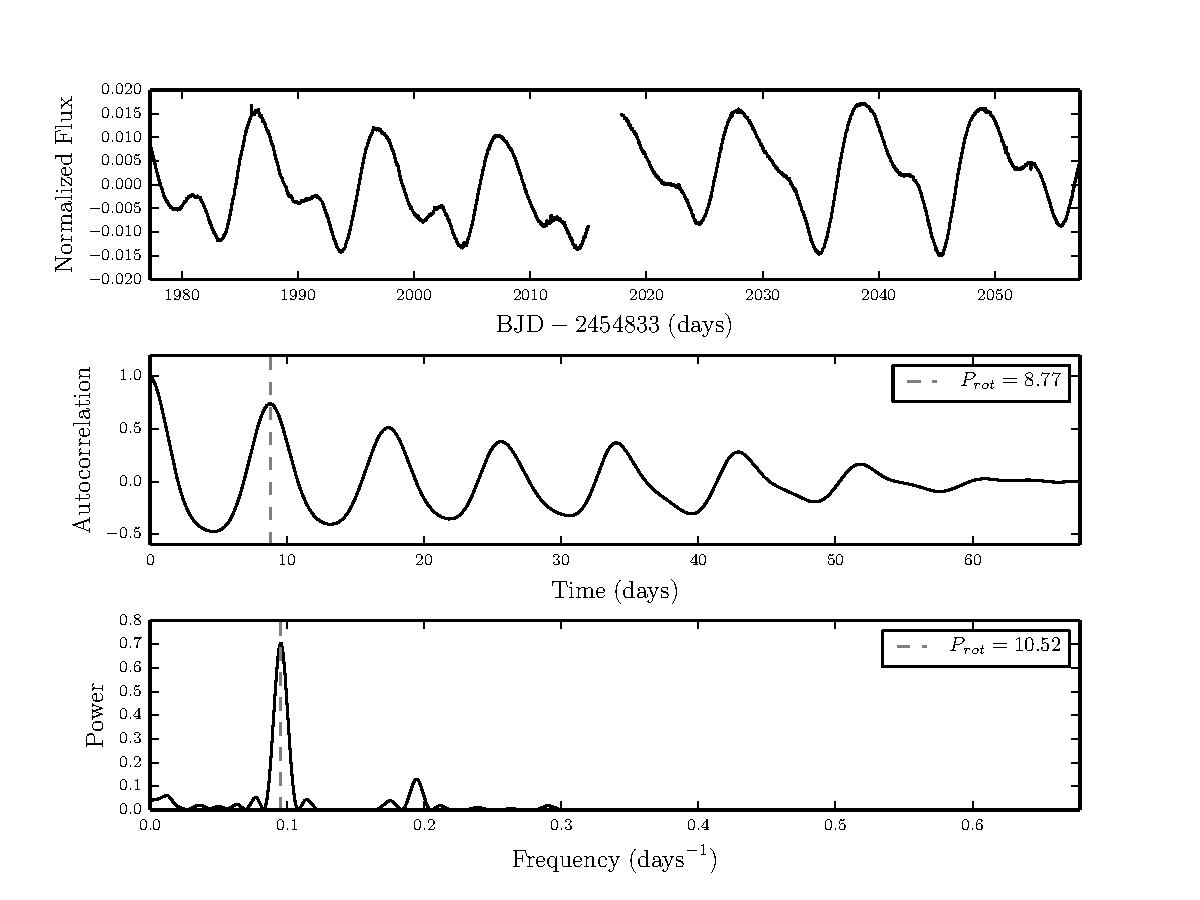
\includegraphics[width=6in, clip=true]{rotation_poster_child.pdf}
\caption{{\it Top}: Light curve of EP201317002, detrended using the method
of \citet{Vanderburg2014}. {\it Middle}: Autocorrelation function of the
light curve. The autocorrelation function method measures a rotation period of
8.77 days for this star. {\it Bottom}: The Lomb-Scargle periodogram of the
light curve. The highest peak in the periodogram is centred at 10.52 days.}
\label{fig:rotation_poster_child}
\end{center}
\end{figure*}

\section{Injections with sinusoids}

In order to test the sensitivity, completeness and reliability of this method
we injected n sinusoids into real {\it K2} light curves.

We generated n sinusoids with periods ranging from blah to blah and injected
these into m raw {\it K2} light curves.
The amplitudes of these sine waves varied from blah to blah ppm.
We then attempted to recover the true periods by computing a periodogram with
simulataneous systematic modelling.
The recovered period is then automatically extracted from the periodogram by
detecting the highest peak.
We say that a period was successfully measured if the recovered period lies
within 10\% of the `truth'.extracted from the periodogram by
detecting the highest peak.

\bibliographystyle{plainnat}
\bibliography{K2rotation}
\end{document}
